\documentclass{beamer}

% \usepackage{beamerthemesplit} // Activate for custom appearance

\title{Price Competition and \\Effects of Political Connections on Allocations:}
\subtitle{Evidence from a Regression Discontinuity in \\Bid-screening Cutoffs for Procurement Auctions}
\author{Yongseok Kim}
\date{\today}

\begin{document}

\frame{\titlepage}

\section{Introduction}

\begin{frame}
\frametitle{Motivation}
\begin{itemize}

\item Previous studies show that political connections can affect procurement allocations (Schoenherr, 2019).
\item However, policy makers often design procurement contracts to be allocated by an auction, which is believed to rule out effects of political connections in a competitive market.
\item Then, how do political connections affect allocations beyond the price competition? This paper aims to answer this question.

\end{itemize}
\end{frame}

\begin{frame}
\frametitle{Motivation}
\begin{itemize}

\item One of suspects is a bid screening: procurers usually disregard abnormally low, ``too-good-to-be-true'' bids and then choose the lowest one among the remaining bids.
\item The rationale for such bid screening practice is that
	\begin{enumerate}
	\item too low bids in construction procurement lead to frequent cost overruns, thereby causing socially wasteful ex-post disputes (Eun, 2019).
	\item weakening collusion by limiting the cartel's ability to punish deviators (Chassang and Ortner, 2017).
	\end{enumerate}
\item Governments of many countries automatize the bid screening process by introducing cutoffs under which bids are disregarded, e.g., Chile, China, Italy, Peru, Switzerland, Taiwan, Japan, and Korea (Decarolis, 2009; Ishii, 2008; Chassang and Ortner, 2017).

\end{itemize}
\end{frame}

\begin{frame}
\frametitle{Motivation}
\begin{itemize}
\item When cutoffs are set properly, ex-ante bid screening reduces the total social cost by reducing ex-post adjustment cost (Eun, 2019).
\item However, such restricted price competition can also lead to increased effects of political connections on a procurement allocation.
	\begin{enumerate}
	\item Minimum price rules can allow procurers to allocate contracts not by bid prices but by political connections or lobbying.
	\item Politically connected CEOs would also have a stronger incentive to utilize their social capital when there is more money on the table.
	\end{enumerate}
\item Though intuitively straightforward, examining this argument is empirically challenging since it requires external variations in restrictions.
\end{itemize}
\end{frame}

\begin{frame}
\frametitle{This Paper}
\begin{itemize}
\item Exploiting a regression discontinuity in bid-screening cutoffs, I suggest a causal evidence supporting this view.
\item Specifically, I use a detailed procurement auction data for military constructions in Korea from 2006 to 2018.
\item Identification:
	\begin{itemize}
	\item Cutoffs are set to be an estimated cost of projects multiplied by a pre-determined ratio.
	\item There is a significant discontinuity in this ratio (5\%) around the estimated cost 10 billion KRW.
	\end{itemize}
\item Assumption: Estimated costs around 10 billion KRW would be randomly distributed.
\end{itemize}
\end{frame}

\begin{frame}
\frametitle{Preview of Findings}
\begin{figure} \centering
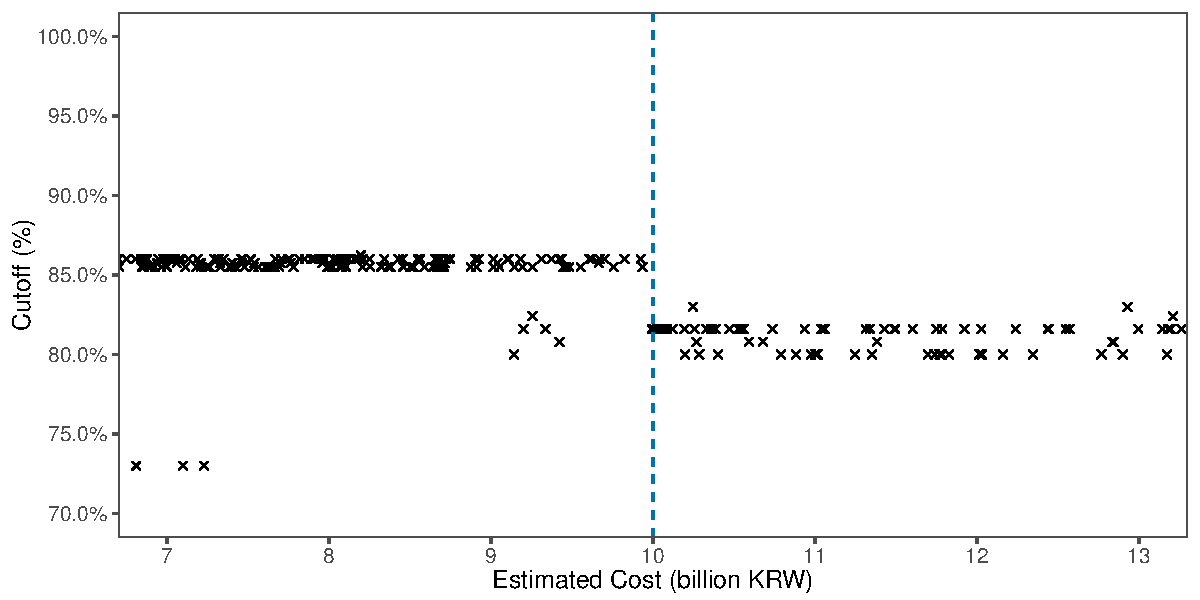
\includegraphics[width = \linewidth]{../figure/limit.pdf}
\caption{Discontinuity in Bid-screening Cutoffs} \label{}
\end{figure}
\end{frame}

\begin{frame}
\frametitle{Preview of Findings}
\begin{figure} \centering
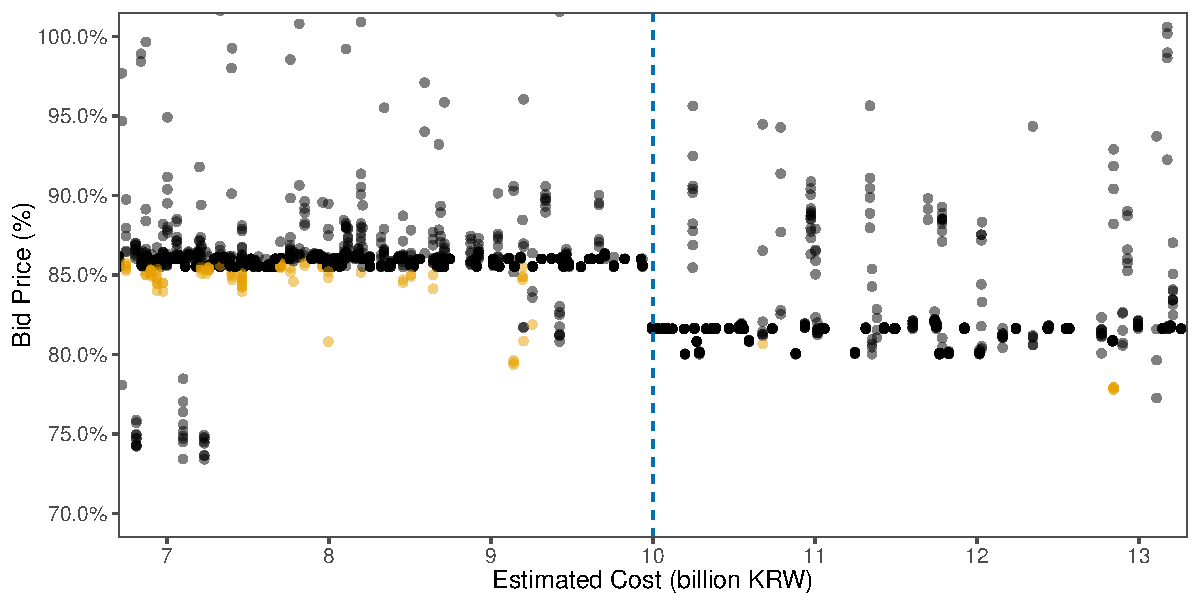
\includegraphics[width = \linewidth]{../figure/bid.pdf}
\caption{Bid Prices Around Cutoffs} \label{}
\end{figure}
\end{frame}

\begin{frame}
\frametitle{Preview of Findings}
\begin{figure} \centering
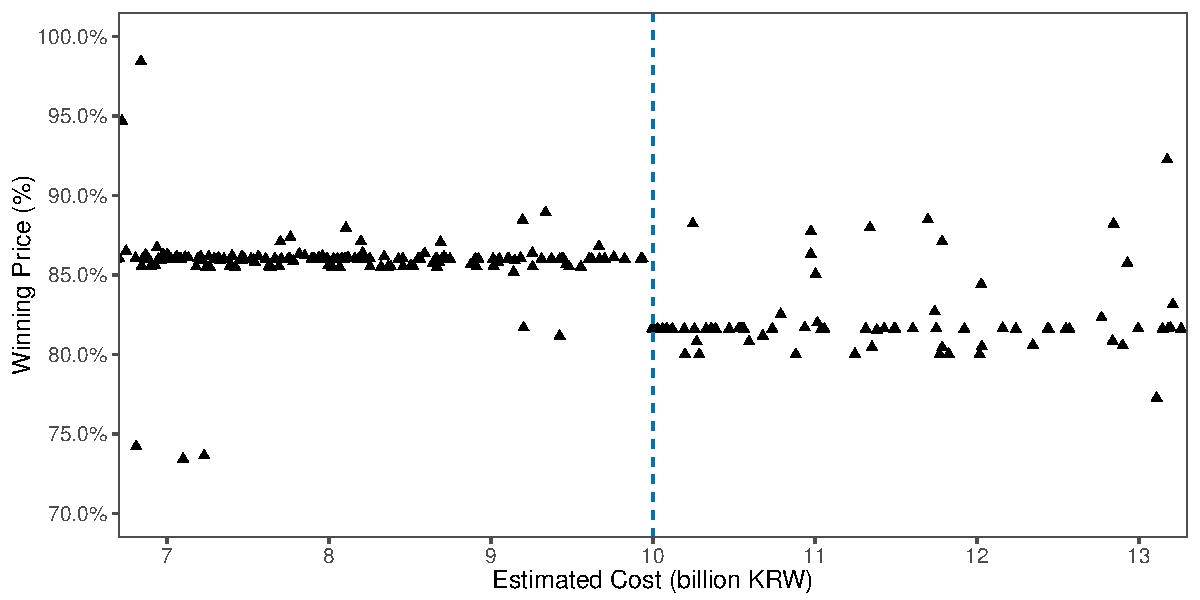
\includegraphics[width = \linewidth]{../figure/win.pdf}
\caption{Winning Prices Around Cutoffs} \label{}
\end{figure}
\end{frame}

\end{document}
